\documentclass[a4paper,12pt]{article}
\usepackage[utf8]{inputenc}
\usepackage{polyglossia}
\setmainlanguage{spanish}
\usepackage{pythonhighlight}
\usepackage{multirow}
\usepackage{booktabs}
\usepackage{enumitem}
\usepackage{amsmath}
\usepackage{amsfonts}
\usepackage{tabularx}
%\usepackage[showframe=true]{geometry}
\usepackage{changepage}
\usepackage{graphicx}
\usepackage{amsmath}
\usepackage{svg}
\usepackage{lscape}
\usepackage[bookmarks = true, colorlinks=true, linkcolor = black, citecolor = black, menucolor = black, urlcolor = black]{hyperref}
%\usepackage[spanish,activeacute]{babel}
\usepackage{lmodern}
\usepackage{listings}
\usepackage{adjustbox}
\usepackage{float}
\renewcommand{\baselinestretch}{1} % Interlineado. 1 es estandar
\usepackage[T1]{fontenc}
\usepackage[square,sort,comma,numbers]{natbib}
\usepackage{mathtools}
\usepackage{fancyhdr}
\fancyhead[R]{2021}\fancyhead[L]{UNC - FCEFyN} \fancyfoot[C]{\thepage}
\pagestyle{fancy}
\usepackage[numbered]{bookmark} % Para que figure las secciones en el PDF
\graphicspath{ {img/} }
\usepackage[normalem]{ulem}
\useunder{\uline}{\ul}{}
\DeclareMathOperator*{\argmax}{arg\,max}
\DeclareMathOperator*{\argmin}{arg\,min}
\author{Gerardo A. COLLANTE \\ Matrícula: 39.022.782 \\ Email: \href{mailto:gerardo.collante@unc.edu.ar}{gerardo.collante@unc.edu.ar} \\ Cel: 54 (03574) 650490}

\begin{document}

\makeatletter
\begin{titlepage}
		
	{\scshape\LARGE Universidad Nacional de Córdoba \par}
	{\Large Facultad de Ciencias Exactas, Físicas y Naturales \par}
	\vspace{0.5cm}
	\centering
	
\includegraphics[width=0.5\textwidth]{unc.png}
	\par\vspace{0.5cm}
	\vspace{0.5cm}
	{\scshape\Large Proyecto Final Integrador\par}
	\vspace{1cm}
	{\large\bfseries ``Predicción de cantidad de defectos graves en vehículos utilitarios en planta automotriz'' \par}
	\vspace{0.5cm}
		
	\textbf{Anexo}
	\vspace{0.5cm}
		
	\normalsize\@author\space
		
	\vspace{0.5cm}
	\textbf{Supervisor}\par
	Dr. Ing.~Orlando \textsc{Micolini}
	
	\vfill
	
	{\large \today\par}
\end{titlepage}

\tableofcontents

\clearpage

\section{Inteligencia Artificial}

\begin{quote}
	La \textit{Inteligencia Artificial (Artificial Intelligence)} se define como el estudio de los "agentes inteligentes", i.e. cualquier dispositivo que perciba su entorno y tome medidas que maximicen sus posibilidades de lograr con éxito sus objetivos.
	  
	\hfill \citet{poole1998}
\end{quote}

Esta definición nos da la idea de que la IA es un sistema reactivo, que reacciona a cambios externos y actúa en consecuencia.

\subsection{Aprendizaje automático} \label{machinelearning}

\begin{quote}
	El \textit{aprendizaje automático (Machine Learning)} es el estudio científico de algoritmos y modelos estadísticos que los sistemas informáticos utilizan para realizar una tarea específica sin utilizar instrucciones explícitas, sino que se basan en patrones e inferencia. Es visto como un subcampo de inteligencia artificial. Los algoritmos de aprendizaje automático crean un modelo matemático basado en datos de muestra, conocidos como "datos de entrenamiento", para hacer predicciones o decisiones sin ser programado explícitamente para realizar la tarea.
	  
	\hfill \citet{bishop2006pattern}
\end{quote}

Es importante destacar la independencia del aprendizaje automático al momento de tomar decisiones a partir de los datos proporcionados sin intervención externa, es decir que no hay una especificación de reglas que dictan cómo deben ser tomadas estas decisiones. A su vez, los modelos obtenidos a partir de los algoritmos de \textit{Machine Learning} deben tener la capacidad de predecir a partir de nuevos datos, nunca antes procesados por el modelo, a esto se lo conoce como \textbf{generalización}. 

\subsection{Preprocesamiento} \label{preprocessing}
Este punto es vital para cualquier proyecto que utiliza algoritmos de \textit{Machine Learning}, debido a que los datos incluidos en los conjuntos conocidos como \textit{datasets}, no suelen presentarse en condiciones para obtener el óptimo rendimiento de los algoritmos de aprendizaje. Estos datos suelen estar desbalanceados, con faltantes o ruidosos, entre otras cuestiones. 

Una vez obtenido el \textit{dataset} de entrada es primordial investigar, limpiar y transformar los datos con diversas técnicas. Una vez que los datos estén en condiciones procedemos al entrenamiento de nuestro modelo, con el propósito de lograr un desempeño óptimo.

Para lograr este objetivo se aplican técnicas tales como normalización, reescalado, reducción de dimensionalidad, discretización, tratamiento de anomalías y \textit{outliers}.

\subsection{Aprendizaje no supervisado} \label{unsupervised}

En este caso no disponemos de una salida deseada, tampoco se disponen datos etiquetados o con estructuras definidas. Por lo que el objetivo principal del Aprendizaje no Supervisado es generar esas etiquetas a partir de la información que se extrae de datos proporcionados en el \textit{dataset}, sin tener una referencia de salida.

Un ejemplo de aprendizaje no supervisado podría ser si nos encontramos con un texto extenso y queremos obtener una especie de resumen, de los temas o tópicos relevantes, probablemente de antemano no se sabe cuales son o su cantidad, por lo tanto nos enfrentamos a la situación de no conocer cuales serian las salidas esperadas del modelo. 
Otros ejemplos clásicos pueden ser agrupar fotografías similares o separación de diferentes fuentes que originan un determinado sonido. 

Como se comentó anteriormente en la sección~\ref{preprocessing}, en la etapa de preprocesamiento, es muy útil aplicar las técnicas del aprendizaje no supervisado ya que se cuentan con grandes cantidades de datos en contextos no conocidos y lo más importante, sin etiquetar. Entonces suele ser una buena práctica dar un primer paso mediante algoritmos de aprendizaje no supervisado antes de pasar los datos a un proceso de aprendizaje supervisado. Como por ejemplo cuando se realizan transformaciones de datos mediante reescalado o estandarización. 

En las próximas subsecciones explicaremos brevemente cada una de las tareas que comprenden el Aprendizaje no Supervisado.

\subsubsection{Detección de anomalías}

Uno de los primeros pasos a realizar cuando se nos presenta un conjunto de datos, es proceder con la tarea llamada detección de anomalías (\textit{anomaly detection}, AD), o identificación de \textit{outliers} o datos fuera de rango. 

Un \textit{outlier} puede ser considerado como un dato atípico en un dataset o que parece ser inconsistente con el resto del conjunto.

\clearpage

Tipos de entornos en los que se produce la detección de anomalías:
\begin{itemize}[noitemsep, topsep=2pt]
	\item AD supervisada:
	      \begin{itemize}[noitemsep, topsep=2pt]
	      	\item Las etiquetas están disponibles, tanto para casos normales como para casos anómalos.
	      	\item En cierto modo, similar a minería de clases poco comunes o clasificación no balanceada.
	      \end{itemize}
	\item AD semi-supervisada (detección de novedades, \textit{Novelty Detection})
	      \begin{itemize}[noitemsep, topsep=2pt]
	      	\item Durante el entrenamiento, solo tenemos datos normales.
	      	\item El algoritmo aprende únicamente usando los datos normales.
	      \end{itemize}
	\item AD no supervisada (detección de \textit{outliers}, \textit{Outlier Detection})
	      \begin{itemize}[noitemsep, topsep=2pt]
	      	\item No hay etiquetas y el conjunto de entrenamiento tiene datos normales y datos anómalos.
	      	\item Asume que los datos anómalos son poco frecuentes.
	      	\item Algunos ejemplos típicos de detección de anomalías pueden ser, cuando se quiere detectar intrusos en tráfico de red o bien detectar acciones fraudulentas en transacciones con tarjetas de crédito.
	      \end{itemize}
\end{itemize}

\begin{figure}[H]
	\begin{center}				
		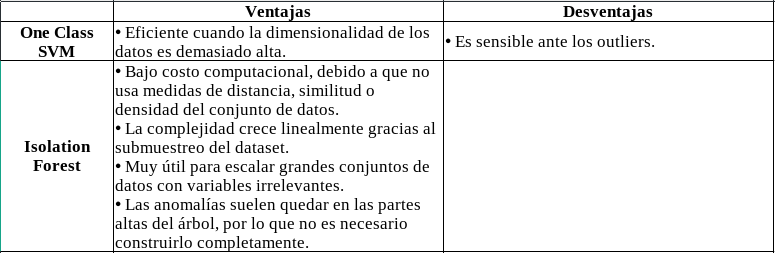
\includegraphics[width=1\textwidth]{tesis_11.png}
		\caption{Ventajas y desventajas de los algoritmos de detección de anomalías.}
		\label{fig:proconsanomaly.}
	\end{center}
\end{figure}

\subsubsection{Reducción de dimensionalidad }

A menudo las muestras disponibles contienen una gran variedad de características, que pueden dar como resultado un sobreajuste del modelo utilizado, por lo tanto es necesario reducir la dimensionalidad de dichos datos pero manteniendo la información relevante. Al reducir la dimensionalidad no solo se evita el sobreajuste, sino que también se obtiene una mejor visualización de los datos y se reduce el costo computacional. 

\clearpage

Uno de los modelos más conocidos y que requieren menor costo computacional es \textit{Principal Component Analysis} (\texttt{PCA}), pero si lo que estamos buscando es una mejor visualización de los datos y además las características no son lineales, sería recomendable usar \texttt{T-SNE}. 

\begin{figure}[H]
	\begin{center}				
		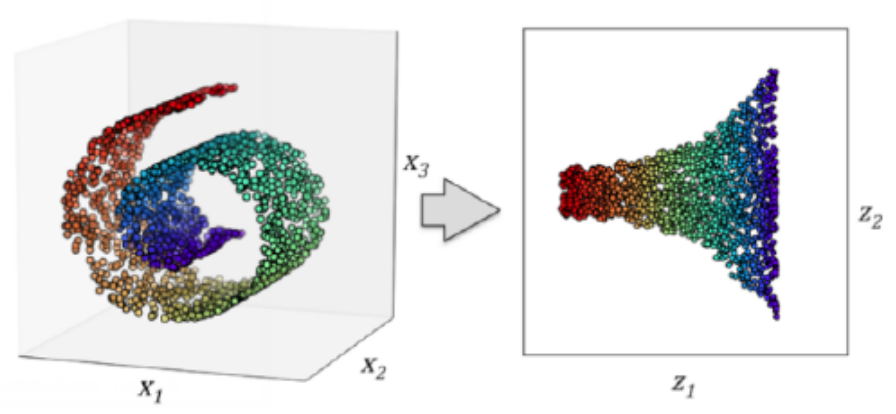
\includegraphics[width=0.7\textwidth]{tesis_12.png}
		\caption{Reducción de dimensionalidad de 3D a 2D.}
		\label{fig:reduxdimension.}
	\end{center}
\end{figure}

En la Fig.~\ref{fig:reduxdimension.} \cite{trejoml} se muestra un ejemplo de cómo la reducción de dimensionalidad facilita la visualización de un dataset de alta dimensionalidad en una proyección de 1, 2 o 3 dimensiones.

Enumeramos en la Fig.~\ref{fig:proconsreduxdim.} las ventajas y desventajas de los algoritmos disponibles para esta tarea.

\begin{figure}[H]
	\begin{center}				
		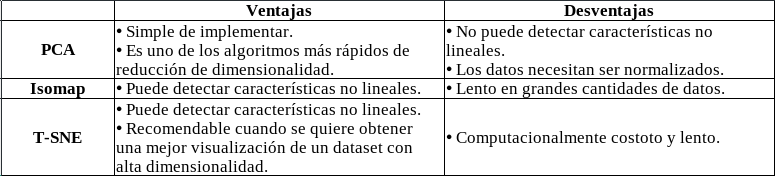
\includegraphics[width=1\textwidth]{tesis_15.png}
		\caption{Pro y contras de algoritmos de reducción de dimensionalidad.}
		\label{fig:proconsreduxdim.}
	\end{center}
\end{figure}

\clearpage

\subsubsection{\textit{Clustering}}

El \textit{clustering} es una técnica que conceptualmente es simple de comprender, consiste en agrupar objetos con características similares. Por lo tanto, obtenemos diferentes grupos llamados clústers, donde en cada uno de ellos están contenidos los datos que son más similares entre ellos que con los que pertenecen a otros clústers, obteniendo de esta forma una útil subdivisión del \textit{dataset}. Como no suele tenerse conocimiento sobre los datos, es decir no están etiquetados, esta técnica pertenece al Aprendizaje no Supervisado.

El algoritmo más simple de \textit{clustering} es K-means, el cual funciona para agrupar datos que se distribuyen en formas esféricas, si se usa la distancia euclídea. y a su vez hay que proporcionar la cantidad k de grupos en los cuales queremos distribuir el \textit{dataset}, por ello se debe tener un conocimiento previo de cuantos clúster se espera tener. 
Otras alternativas pueden ser, realizar \textit{clustering} jerárquico o \textit{clustering} basados en densidades.

En \textit{clustering} jerárquico, vemos como resultado un dendograma, es decir un diagrama de árbol. A partir de esto, se decide un umbral de profundidad, donde se corta el árbol y  de esta forma se obtiene un agrupamientos, por lo tanto a diferencia con K-means, no necesitamos tener información para poder decidir la cantidad de grupos. En la Fig.~\ref{fig:dendogram.} podemos observar como quedan evidenciados a través del dendograma los diferentes clusters.

\begin{figure}[H]
	\begin{center}				
		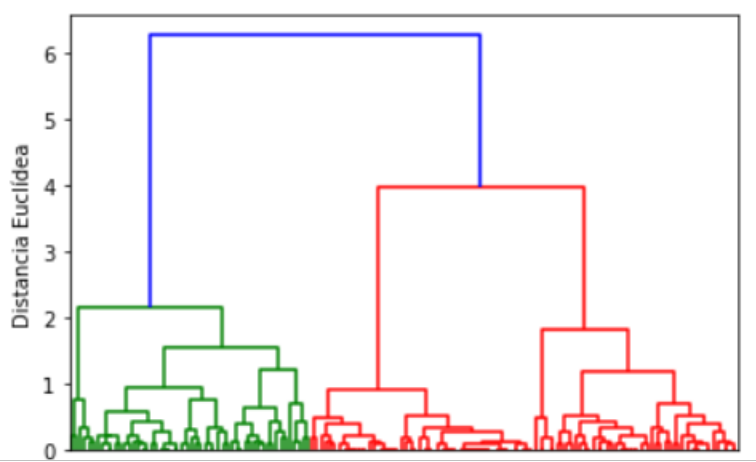
\includegraphics[width=0.6\textwidth]{tesis_16.png}
		\caption{Dendograma generado por \textit{clustering} jerárquico.}
		\label{fig:dendogram.}
	\end{center}
\end{figure}

En cambio DBSCAN (\textit{Density-based Spatial Clustering of Applications with Noise}), divide el \textit{dataset} buscando las regiones densas de puntos, como podemos observar claramente en Fig.~\ref{fig:DBSCAN.}. Con esta técnica, tampoco especificamos el número de parámetros a priori, sino que se establecen hiperparámetros adicionales, como lo son la cantidad mínima de puntos y un radio $\epsilon$, para lograr un óptimo funcionamiento.

\begin{figure}[H]
	\begin{center}				
		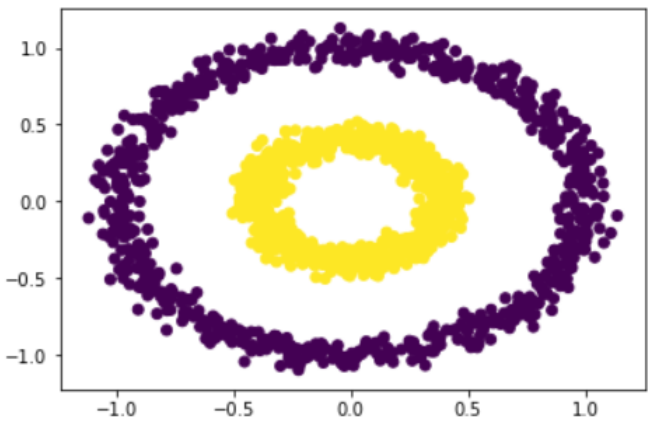
\includegraphics[width=0.6\textwidth]{tesis_17.png}
		\caption{Clustering basado en densidades.}
		\label{fig:DBSCAN.}
	\end{center}
\end{figure}

Enumeramos en la Fig.~\ref{fig:proconsclustering.} las ventajas y desventajas de los algoritmos disponibles para esta tarea.

\begin{figure}[H]
	\begin{center}				
		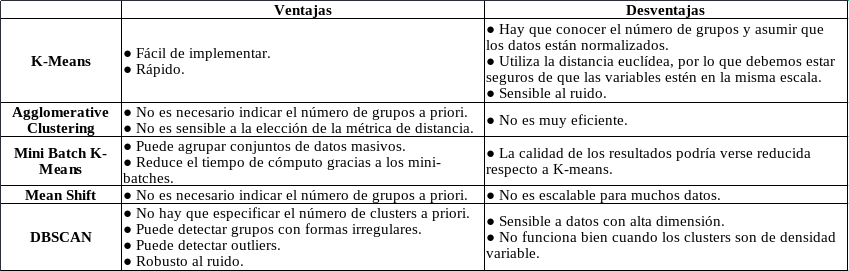
\includegraphics[width=1\textwidth]{tesis_34.png}
		\caption{Pros y contras de los algoritmos de \textit{clustering}.}
		\label{fig:proconsclustering.}
	\end{center}
\end{figure}

\clearpage

\subsection{Selección de algoritmo en base al \textit{dataset}}
En la Fig.~\ref{fig:maindiagram.} obtenemos una vista general sobre que hacer con nuestros datos en función a nuestro objetivo.

\begin{figure}[H]
	\begin{center}				
		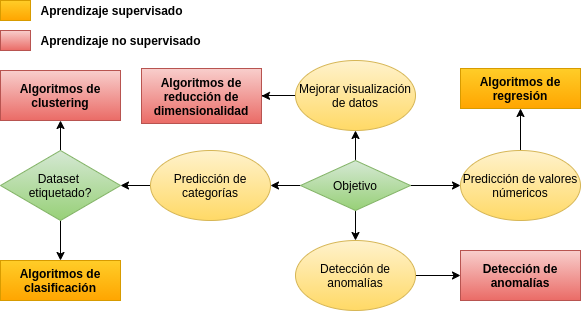
\includegraphics[width=1\textwidth]{maindiagram.png}
		\caption{Diagrama general de algoritmos de aprendizaje supervisado y no supervisado.}
		\label{fig:maindiagram.}
	\end{center}
\end{figure}

\subsubsection{Algoritmos no supervisados}

\begin{figure}[H]
	\begin{center}				
		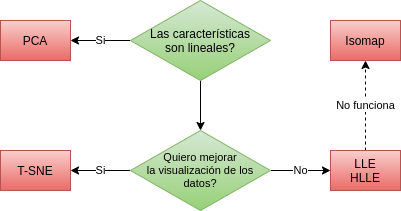
\includegraphics[width=0.8\textwidth]{dimreduxdiagram.png}
		\caption{Diagrama general de los algoritmos de reducción de dimensión.}
		\label{fig:dimreduxdiagram.}
	\end{center}
\end{figure}

\begin{figure}[H]
	\begin{center}				
		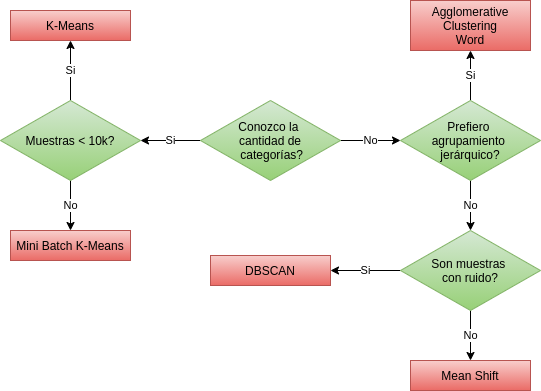
\includegraphics[width=0.9\textwidth]{clusteringdiagram.png}
		\caption{Diagrama general de los algoritmos de \textit{clustering}.}
		\label{fig:clusteringdiagram.}
	\end{center}
\end{figure}

\begin{figure}[H]
	\begin{center}				
		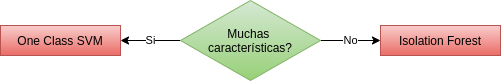
\includegraphics[width=0.9\textwidth]{anomalydiagram.png}
		\caption{Diagrama general de los algoritmos de detección de anomalías.}
		\label{fig:anomalydiagram.}
	\end{center}
\end{figure}

\clearpage

\setcounter{page}{13}

\begin{landscape}
		
	\begin{table}[]
		\centering
		\begin{tabularx}{\hsize}{|X|X|X|}
			\hline
			\multicolumn{1}{|c|}{\textbf{Algoritmo}} & \multicolumn{1}{|c|}{\textbf{Ventajas}} & \multicolumn{1}{|c|}{\textbf{Desventajas}} \\
			\hline
			\textit{Naive Bayes}   & 
			- No necesita una gran cantidad de datos de entrenamiento. 
						
			- Rápido. & 
			- Supone que cada característica es independiente. 
						
			- Sufre al tener características irrelevantes.
			\\ \hline
			Regresión logística      & 
			- Rara vez existe sobreajuste. 
						
			- Rápido de entrenar. & 
			- Es muy difícil lograr que se ajuste a datos no lineales. 
						
			-Los valores atípicos alteran la precisión del modelo. 
						
			\\ \hline
			\textit{KNN}           & 
			- Eficaz en \textit{datasets} de varias clases. 
						
			- Entrenamiento rápido. & 
			- La dimensionalidad del \textit{dataset} merma el rendimiento.
						
			- Lento en inferencia. 
			\\ \hline
			Árbol de decisión 
						
			\textit{(Decision Tree)} & 
			- Robusto en muestras con ruido. 
						
			- Fácil interpretación. 
						
			- Resuelve problemas no lineales. & 
			- Cuando hay muchas etiquetas de clases, los cálculos pueden ser complejos. 
						
			- Puede sufrir sobreajuste. 
			\\ \hline
			Clasificador de bosque aleatorio 
						
			\textit{(Random Forest Classifier)} & 
			- No sufre sobreajuste como el árbol de decisión. 
						
			- Funciona muy bien en grandes \textit{datasets}. 
						
			- Maneja automáticamente los valores faltantes. & 
			- Consume mucho tiempo y recursos computacionales.
						
			- Difícil de interpretar.
						
			- Se debe elegir la cantidad adecuada de árboles.
			\\ \hline
			Máquinas de vectores de soporte 
						
			\textit{(Support Vector Machines)}  & 
			- Eficaz en espacios de gran dimensión.
						
			- Puede manejar soluciones no lineales.
						
			- Robusto al ruido.
			& 
			- Lento para entrenarse con grandes conjuntos de datos. 
						
			- Ineficaz si las clases se superponen.
						
			- Se debe elegir correctamente la función de \textit{kernel}.
						
			- Difícil de interpretar al aplicar \textit{kernels} no lineales.
			\\ \hline
		\end{tabularx}
		\caption{Pros y contras de cada algoritmo supervisado.}
		\label{tab:pro-cons-supervised}
	\end{table}
		
\end{landscape}


\begin{landscape}

	\setcounter{page}{15}
		
	\begin{table}[]
		\centering
		\begin{tabularx}{\hsize}{|X|X|X|}
			\hline
			\multicolumn{1}{|c|}{\textbf{Algoritmo}} & \multicolumn{1}{|c|}{\textbf{Ventajas}} & \multicolumn{1}{|c|}{\textbf{Desventajas}} \\
			\hline
			\textit{Ridge}   & 
			- El costo computacional no es mayor que otros algoritmos.
						
			- Permite evitar el sobreajuste. & 
			- Se necesita una excelente selección del hiperpaŕametro $\alpha$. 
						
			- Incrementa el sesgo.
			\\ \hline
			\textit{LASSO}      & 
			- Evita el sobreajuste. 
						
			- Selecciona características tendiendo a que sus coeficientes sean 0. & 
			- Las características seleccionadas tienen demasiado sesgo. 
						
			- Si tenemos $n$ datos y $p$ características, \textit{LASSO} solo selecciona como máximo $n$ características. 
						
			- El rendimiento de la inferencia es peor que para \textit{Ridge}.
						
			\\ \hline
			\textit{ElasticNet}           & 
			- Eficaz con muestras de gran dimensión.
			& 
			- Alto costo computacional en comparación a \textit{LASSO} o \textit{Ridge}.
			\\ \hline
			\textit{KNN Regressor} & 
			- No tiene período de entrenamiento.
						
			- Fácil interpretación.
						
			- Permite agregar datos al modelo sin inconvenientes en la precisión del algoritmo.
			&
			- La dimensionalidad del \textit{dataset} influye mucho en el rendimiento.
						
			- Es sensible a datos ruidosos, valores faltantes y \textit{outliers}.
						
			- En grandes \textit{datasets} se vuelve muy alto el costo computacional para calcular distancias.			
						
			\\ \hline
			Regresor de árbol de decisión
						
			\textit{(Decision Tree Regressor)} & 
			- No sufre sobreajuste como el árbol de decisión.
						
			- Funciona muy bien en grandes \textit{datasets}. 
						
			- Maneja automáticamente los valores faltantes. & 
			- Al trabajar con variables continuas, se pierde mucha información al categorizar.
						
			- Necesita variables correlacionadas.
						
			- Alto tiempo de entrenamiento.
						
			- Se puede volver demasiado complejo.
			\\ \hline
			Máquinas de vectores de soporte 
						
			\textit{(Support Vector Machines)}  & 
			- Útil cuando las clases no son linealmente separables.
			& 
			- Suelen ser ineficientes al momento del entrenamiento.
			\\ \hline
		\end{tabularx}
		\caption{Pros y contras de cada algoritmo supervisado.}
		\label{tab:pro-cons-supervised}
	\end{table}
		
\end{landscape}

\bibliography{tesis}{}
\bibliographystyle{unsrtnat}

\end{document}